\chapter{Regolith amplification}
\label{ch:reg}


\section{Overview}

Regolith is defined as the soil, geological sediments and
weathered rock that overly the un-weathered bedrock. It is well
documented that the presence of regolith can increase the level of
ground shaking experienced during an earthquake
(\citealt{dr_Borcherdt76a}; \citealt{dr_Murphy71a}).  For example,
studies in the San Fernando Valley and Los Angeles Basin, U.S.A.,
have demonstrated that the damage patterns observed during the
1994 Northridge, California earthquake can be strongly correlated
to site-response of local regolith \citep{dr_Meremonte96a}.
Consequently, including the effect of regolith on earthquake
ground shaking is an important component of any seismic hazard or
risk analysis.

\subsection{Background theory}

An amplification factor can be used to transfer the earthquake
motion from the bedrock to the regolith surface. Amplification
factors are influenced by the regolith at the site of interest,
the magnitude $r_m$ of the event and the PGA for the event-site
combination. For simplicity, the geographical region of interest
is usually separated into five or six site-classes inside which
the regolith is assumed to be the same. The EQRM application does
not compute the amplification factors (or level of amplification).
Such calculations must be conducted off-line and the results (or
amplification factors) made available to the EQRM application. The
interested reader is referred to \citet{dr_Robinson06a} for a
detailed description of the equivalent linear technique for
computing amplification factors. \citet{dr_Dhu02b} discuss the
classification of site classes and the application of
amplification factors to a probabilistic seismic hazard analysis.
\fref{fig:regolith-newcexample-crosssection} illustrates the
geotechnical cross section for all of the site classes in the
Newcastle and Lake Macquarie region, and
\fref{fig:regolith-newcexample-ampfactors} shows an example of the
amplification factors use in the same study.


\begin{figure}
\begin{center}
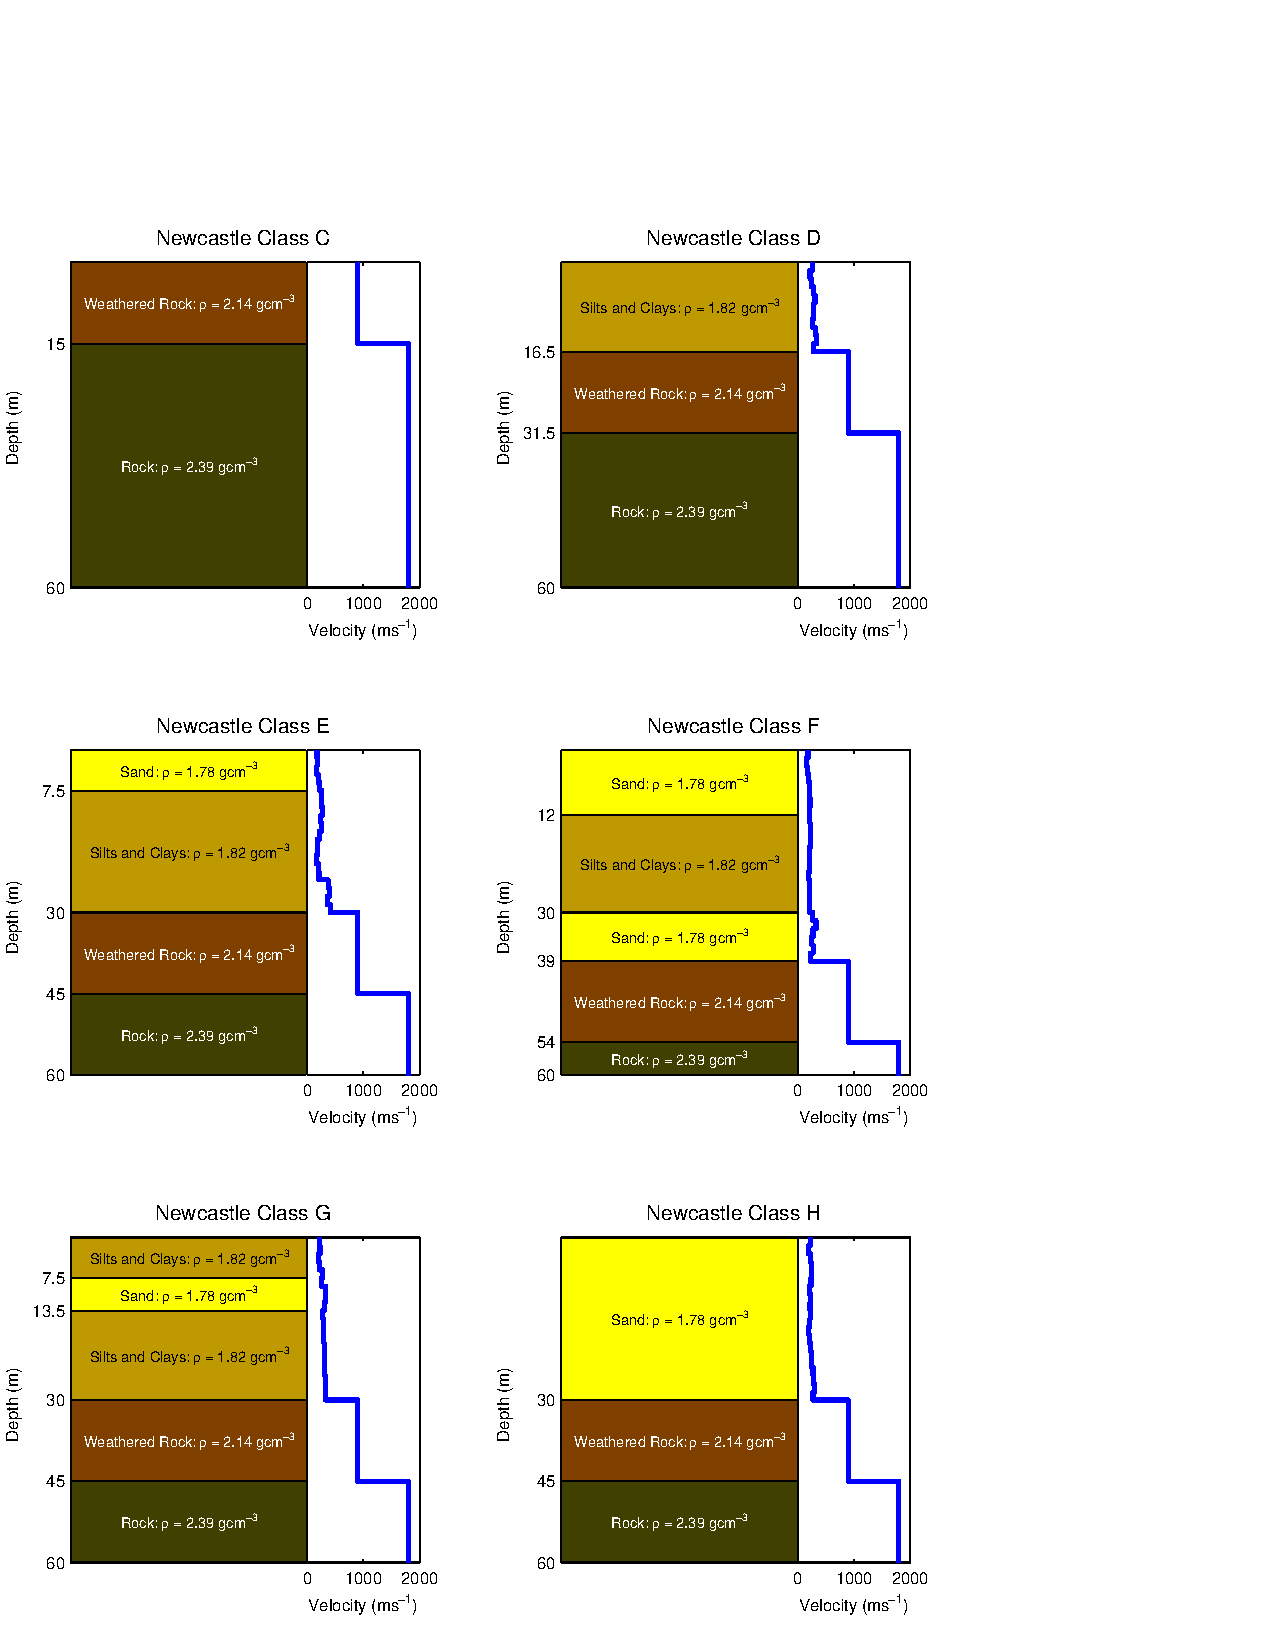
\includegraphics[width=0.6\textheight]{fig-hregolith-crosssections}
\end{center}
\caption{Cross sections of the 6 site classes used in the
Newcastle and Lake Macquarie study \citep{dr_Dhu02b}. }
\label{fig:regolith-newcexample-crosssection}
\end{figure}

\begin{figure}
\begin{center}
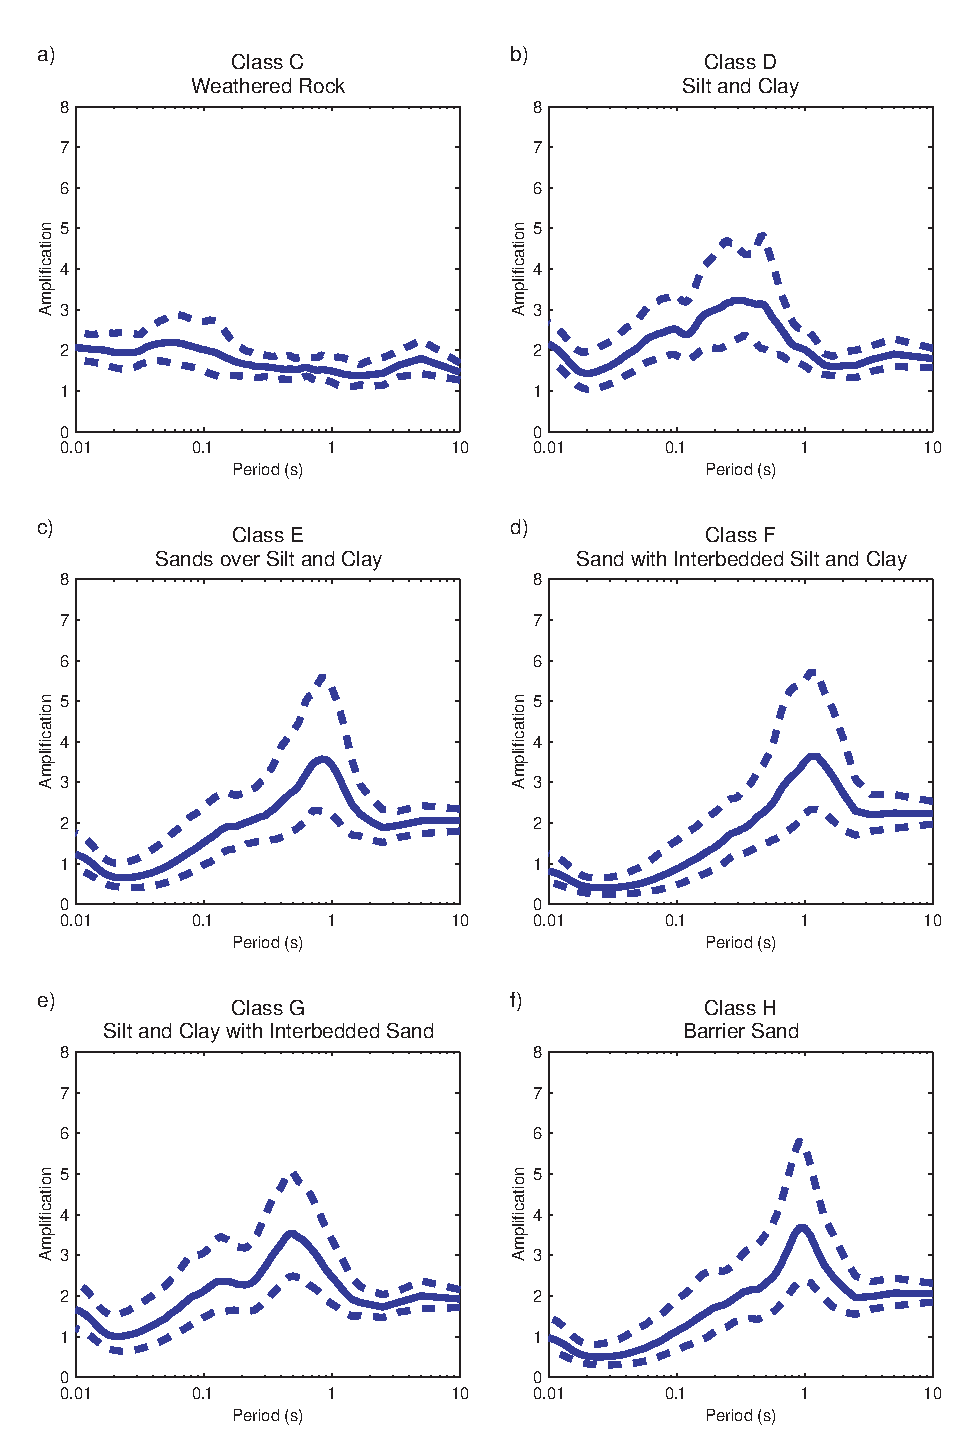
\includegraphics[width=0.6\textheight]{fig-hregolith-ampfactors}
\end{center}
\caption{Example amplification factors for the site classes shown
in \fref{fig:regolith-newcexample-crosssection}. Note that the
amplification factors are for moment magnitude 5.5 and PGA
$0.25g$. } \label{fig:regolith-newcexample-ampfactors}
\end{figure}


\section{Implementation}

As with the attenuation, the implementation of the amplification
factors (for both hazard and risk assessments) has been done in a
two step process as follows:
\begin{enumerate}
\item The preparation of the amplification factors
conducted before entering a loop over sites. \item Application of
the amplification factors to compute $A_{S_a,soil}(T_o,r_m,R)$ at
each site conducted within a loop over sites.
\end{enumerate}

The preparation of amplification factors involves interpolating each
to the periods defined in the the EQRM control file parameter (see
~\sref{sec:application-EQRMcf}). The application of the
amplification factors is carried out immediately after the
evaluation of the attenuation model. The process is described for a
specific site located within a known Site Class:
\begin{enumerate}
\item Bin all of the events in the event catalogue into the
bedrock PGA and moment magnitude bins defined by the bin centroids
(see ~\sref{sec:-appl-amplification}). Note that the end points of
the 'central' bins are assumed to be half way between the bin
centroids. The first and last bins extend to negative and positive
infinity respectively.
\item Use a nested loop over all PGA bins (upper loop) and moment
magnitude bins (lower loop) and apply the amplification factor as
follows:
\begin{equation}
S_{a,soil}(T_o,r_m,R)= F_{amp}(T_o,r_m^*,PGA^*) \times
S_{a,bedrock}(T_o,r_m,R),
\end{equation}
where $r_m^*$ and $PGA^*$ are the centroids of the bins containing
$r_m$ and \newline $S_{a,bedrock}(0,r_m,R)$ respectively. The
$F_{amp}$ represents the exponential of `some selection' of
amplification factor from the distribution \newline \mbox{$N \sim
(\mu_{log(F)}(T_o,r_m^*,PGA^*),\sigma_{log(F)}(T_o,r_m^*,PGA^*))$}.
The actual selection  made will depend on the method used to
incorporate uncertainty (see \sref{sec:regolith-incorp-unc}).
\end{enumerate}
Notice that the use of $N \sim (\mu_{log(F)},\sigma_{log(F)})$
equates to the assumption that the amplification factors are
log-normally distributed.

\section{Incorporating aleatory uncertainty}
\label{sec:regolith-incorp-unc}


In theory, both the random selection and PDF sampling methods
described in \sref{attn:uncertainty} could be used to incorporate
aleatory uncertainty in amplification factors. Some care will need
to be taken if the PDF sampling technique is to be used for
incorporating uncertainty at several levels  of computation (e.g.
for attenuation and amplification) due to the need to spawn the
event catalogue (see \sref{source:spawning}) at every level. Such
iterative spawning may lead to a `blow-out' in the size of the event
catalogue and hence the computation time. Currently only the random
selection technique is available for use with the amplification
factors in the EQRM application.

As with the application of an attenuation model, the EQRM applies
$PGA_{cut}$ to $S_{a,soil}(T_o,r_m,R)$ after applying the
amplification factor. This accounts for any unrealistically high
selection of amplification factor. A secondary upper cut-off
facility exists and involves the use of the amplification maximum
factor (AmaxF) (see \sref{sec:application-EQRMcf}). The AmaxF
parameter is applied directly to the amplification factor as
follows:
\begin{equation}
\label{eq:regolith-maxampfactor}
F_{new}(T_o,r_m^*,PGA^*) = \left \{ \begin{array}{ll} F_{old} & \textrm{$\forall$ \hspace{0.2em} $T_o$ s.t. $F_{amp,old}< $ AmaxF} \\
\textrm{AmaxF} & \textrm{$\forall$ \hspace{0.2em} $T_o$ s.t. $F_{amp,old} \geq $ AmaxF} \\
\end{array} \right.
\end{equation}
or brevity the functional reference to $r_m^*$ and $PGA^*$ in
$F_{new}$ and $F_{old}$ in
\ereftwo{eq:regolith-maxampfactor}{eq:regolith-minampfactor} refers
to the fact that these values represent the bin centroids of
magnitude and PGA bins, respectively. In most simulations the
secondary cutoff is not used since $PGA_{cut}$ handles scaling for
an upper bound. Ignoring AmaxF is achieved by setting it to to a
very high number (e.g. AmaxF=10000). In contrast, there is another
parameter in the EQRM control file known as amplification minimum
factor (AminF) which is commonly utilised within the EQRM
application (see \sref{sec:application-EQRMcf}). This parameter
stops the selection of any unrealistically low selections of the
amplification factor. The AminF is commonly set to around 0.6. It is
applied as follows:
\begin{equation}
\label{eq:regolith-minampfactor}
F_{new}(T_o,r_m^*,PGA^*) = \left \{ \begin{array}{ll} F_{old} & \textrm{$\forall$ \hspace{0.2em} $T_o$ s.t. $F_{amp,old} > $ AminF} \\
\textrm{AminF} & \textrm{$\forall$ \hspace{0.2em} $T_o$ s.t. $F_{amp,old} \leq $ AminF} \\
\end{array} \right.
\end{equation}
Note that a value of \mbox{$F<1$} leads to a de-amplification of
the bedrock motion.
